%!TEX program = xelatex
% 完整编译: xelatex -> biber/bibtex -> xelatex -> xelatex
\documentclass[lang=cn,a4paper,newtx]{elegantpaper}
\usepackage{algorithm}
\usepackage{algorithmicx}
\usepackage{algpseudocode}
\usepackage{subfig}
\usepackage{longtable}
\usepackage{lipsum}
\usepackage{makecell}
\usepackage{siunitx}
\usepackage{tikz-timing}
\usepackage{tikz}
\usepackage[table]{xcolor}
% \usepackage[backend=biber,style = gb7714-2015]{biblatex}
\addbibresource{reference.bib} % 参考文献,不要删除
\renewcommand{\listtablename}{表格目录}
\renewcommand{\appendixname}{附录~\Alph{section}}

\lstdefinelanguage{Assembly}{
  morekeywords={ ADD, SUB, MPY, JGZ, JMP, AND, OR,BUT,LOAD,STORE,SHIFTL,SHIFTR,HALT},  % 你可以在这里添加更多汇编指令
  sensitive=true,  % 保证区分大小写
  morecomment=[l]; % 单行注释(以分号开始)
  morestring=[b]",  % 字符串用双引号括起来
}
% Define the style for listings
\lstset{
  language=Verilog,  % 选择使用的语言
  basicstyle=\ttfamily\small,  % 基础字体风格
  keywordstyle=\color{blue}\bfseries,  % 指令的颜色和加粗
  commentstyle=\color{gray},  % 注释的颜色
  stringstyle=\color{red},  % 字符串的颜色
  identifierstyle=\color{purple},  % 标识符的颜色
  backgroundcolor=\color{lightgray!10}, % 背景色
  numbers=left,  % 行号显示在左侧
  stepnumber=1,  % 每行显示一个行号
  numberstyle=\tiny\color{gray},  % 行号的字体样式
  numbersep=5pt,  % 行号与代码之间的间距
  breaklines=true,  % 自动换行
  showstringspaces=false,  % 不显示字符串中的空格
  columns=flexible,  % 调整列宽
  frame=single,  % 在代码块外部加一个框
  framerule=0.5mm,  % 框线宽度
  rulesepcolor=\color{black},  % 分隔线颜色
  captionpos=b,  % 标题位置(b: bottom)
  }


  \tikzset{
  timing/name/.cd,
  I/.style={fill=blue!20},    % IF阶段
  D/.style={fill=green!20},   % ID阶段
  F/.style={fill=red!20},     % FO阶段
  N/.style={fill=yellow!20},  % IND阶段
  E/.style={fill=orange!20},  % EX阶段
  W/.style={fill=purple!20}   % WB阶段
}
% \renewcommand{\refname}{参考文献}
\title{计算机组织与结构II:CPU设计文档}
\author{李勃璘 \\ 吴健雄学院}

\version{1.1}
\date{\zhdate{2025/4/14}}

% 本文档命令
\usepackage{array}
\newcommand{\ccr}[1]{\makecell{{\color{#1}\rule{1cm}{1cm}}}}



\begin{document}

\maketitle
\thispagestyle{empty}
\begin{abstract}

\end{abstract}

% Removed
% \vspace{1cm}

% \textbf{版本更新记录:}

% \begin{longtable*}{|c|c|p{10cm}|}
%   \hline
%   \textbf{版本号} & \textbf{日期} & \textbf{更新内容} \\
%   \hline
%   \endfirsthead

%   \hline
%   \textbf{版本号} & \textbf{日期} & \textbf{更新内容} \\
%   \hline
%   \endhead

%   v1.0 & 2025-03-22 & 初始版本,包含基本 CPU 设计框架,流水线结构,Verilog 实现。 \\
%   \hline
%   v1.1 & 2025-03-29 & 修改 \\

% \end{longtable*}


\newpage
\pagenumbering{roman}
\tableofcontents
\newpage
\listoftables
\newpage
\pagenumbering{arabic}
\section{概述}
\lipsum[5]\footnote{手搓CPU是人类文明的伟大工程 —— 沃兹基硕德}

\subsection{时间安排}
文献\cite{timeline}设计并实施了一个基于FPGA的五级流水线MIPS CPU课程项目,通过阶段性进度安排和动手实践,有效提升了学生对计算机体系结构的理解和项目完成率。受该工作的启发,本文针对本项目制定了工作安排如表所示。
\section{CPU结构设计}
\subsection{总体架构}
CPU由控制单元(CU),逻辑运算单元(ALU),内存(Memory)和寄存器组(Registers)组成,除内存以外,其余单元由被CU生成的控制信号控制的数据通路(Data Path)连接。另外,MAR和MBR分别还和地址总线、数据总线相连接,用于与内存交互。控制单元和内存都和控制总线相连接,用于与外部控制信号交互。

为简单起见,CPU的计算全部为\textbf{16位定点有符号数计算}。

\textcolor{blue}{这里需要一张图!!!}




\subsection{指令集架构}
指令集是指CPU能够对数据进行的所有操作的集合。每一条指令都可以被解释为寄存器与寄存器、内存、I/O端口之间的交互。交互方式由CU中的微指令(Micro-operation)给出,且每一条微指令都需要一个时钟执行(如不进行优化)。
\subsubsection{位宽设计}
地址段长为\textbf{8}位,指令码(Opcode)宽度为\textbf{8}位。因此,每一条指令的位宽为\textbf{16}位。
\subsubsection{寻址方式}
寻址方式指对地址段数据的解释方式。寻址方式由对应指令指定,支持表~\ref{tab:ISA:addressingmode}~中的全部寻址方式。由于给定的指令集高四位均空闲,使用最高位存储支持的寻址方式。目前设计中指令码的最高位为1时,寻址方式为立即数寻址;指令码的最高位为0时,寻址方式为直接寻址。
\begin{longtable}{c c c}
  \caption{指令集支持的寻址方式} \label{tab:ISA:addressingmode} \\
  \toprule
  寻址方式  & 描述 & 最高位\\
  \midrule
  \endfirsthead
  
  \caption[]{(续表)指令集支持的寻址方式} \\
  \toprule
  寻址方式  & 描述 & 最高位\\
  \midrule
  \endhead
  
  \midrule
  \multicolumn{3}{r}{续下页} \\
  \midrule
  \endfoot
  
  \bottomrule
  \endlastfoot
  
  立即数寻址   &  地址字段是操作数本身,数据为补码格式  & 1\\
  直接寻址 &  地址字段为存放操作数的地址    & 0\\
\end{longtable}

\subsubsection{指令集支持的指令}
指令集共支持13条不同的指令,列于表~\ref{tab:ISA:instructions}。每一条指令包含一个指令码,使用二进制格式存储。\footnote{指令中含*的仅支持直接寻址,因为立即数寻址对这些指令无意义。含$^\circledast$的仅支持立即数寻址。}
  


\begin{longtable}{c c c}
  \caption{指令集包含指令及功能} \label{tab:ISA:instructions} \\
  \toprule
  助记符  & 指令码(低四位) & 描述 \\
  \midrule
  \endfirsthead
  
  \caption[]{(续表)指令集包含指令及功能} \\
  \toprule
  助记符  & 指令码(低四位) & 描述 \\
  \midrule
  \endhead
  
  \midrule
  \multicolumn{3}{r}{续下页} \\
  \midrule
  \endfoot
  
  \bottomrule
  \endlastfoot
  
  *STORE X &  0001   & 结果存入\textbf{数据地址}X \\
  *LOAD X  & 0010    & 加载\textbf{数据地址}X \\
  ADD X   & 0011    & 定点数加法\\
  SUB X   & 0100  & 定点数减法\\
  $^\circledast$JGZ X   & 0101    & 结果 > 0时跳转至\textbf{指令地址}X\\
  $^\circledast$JMP X   & 0110    & 无条件跳转至\textbf{指令地址}X\\
  HALT    & 0111    & 暂停程序\\
  MPY X   & 1000    & 定点数乘法 \\
  AND X   & 1001    & 按位与\\
  OR X    & 1010    & 按位或\\
  NOT X   & 1011    & 按位非 \\
  $^\circledast$ SHIFTR X & 1100    & 算术右移 X 位\\
  $^\circledast$ SHIFTL X & 1101    & 算术左移 X 位\\
\end{longtable}

\subsection{CPU内部寄存器}
该部分描述CPU内部寄存器的含义、存储格式和数据被解释为的格式。这些寄存器通过CPU的内部数据通路相连接。寄存器操作是CPU快速操作的核心。

\begin{longtable}{c c c c c c}
  \caption{CPU内部寄存器的含义、总存储条数、单位位宽和数据解释格式} \label{tab:CPU:datawidth} \\
  \toprule
  寄存器 & 含义 & 条数 & 位宽 & 数据解释格式 & 归属模块\\
  \midrule
  \endfirsthead

  \caption[]{(续表)CPU内部寄存器的含义、总存储条数、单位位宽和数据解释格式} \\
  \toprule
  寄存器 & 含义 & 条数 & 位宽 & 数据解释格式 & 归属模块\\
  \midrule
  \endhead

  \midrule
  \multicolumn{6}{r}{续下页} \\
  \midrule
  \endfoot

  \bottomrule
  \endlastfoot

  PC   & 程序计数器,存储当前指令地址             & 1  & 8   & 指令码(Opcode) & /\\
  MAR  & 内存地址寄存器,存储要访问的内存地址     & 1  & 8   & 地址码(Address)& /\\
  MBR  & 内存缓冲寄存器,存储从内存读取或写入的数据 & 1  & 16  & 二进制补码 & /\\
  IR   & 指令寄存器,存储当前正在执行的指令       & 1  & 8   & 指令码(Opcode)& /\\
  BR   & 寄存器,存储 ALU 计算结果        & 1  & 32  & 二进制补码 & ALU\\
  ACC  & 累加寄存器,存储 ALU 运算结果           & 1  & 16  & 二进制补码 & ALU\\
  MR   & 乘法寄存器,存储 ALU 乘法高 16 位       & 1  & 16  & 二进制补码 & ALU\\
  CM   & 控制存储器,存储微指令控制信号         & 未定 & 14  & 控制信号 & CU\\
  CAR  & 控制地址寄存器,指向当前执行的微指令   & 1  & 4   & CM中的条数下标 & CU\\
  CBR  & 控制缓冲寄存器,存储当前微指令的控制信号 & 1  & 14  & 控制信号 & CU\\
\end{longtable}

除上述寄存器以外,ALU进行运算时还会更改\textbf{状态寄存器}(Flags),用于CU进行条件判断。例如,JGZ命令需要判断上一步的运算结果是否是0,CU可以直接通过状态寄存器中的ZF(Zero Flag)寄存器直接进行判断。本设计中使用的所有状态寄存器见表~\ref{tab:CPU:status},它们都直接连向CU,通路不受控制信号的控制。

\begin{longtable}{c c c}
  \caption{状态寄存器列表} \label{tab:CPU:status} \\
  \toprule
  寄存器 & 全称 & 行为 \\ 
  \midrule
  \endfirsthead

  \caption[]{(续表)状态寄存器列表} \\
  \toprule
  寄存器 & 全称 & 行为\\
  \midrule
  \endhead

  \midrule
  \multicolumn{3}{r}{续下页} \\
  \midrule
  \endfoot

  \bottomrule
  \endlastfoot

  ZF   & Zero Flag             & ALU运算结果(通常为ACC)为0时置1\\
  CF  & Carry Flag     & 存储算术移位移出的比特(由于有符号数不存储进位)\\
  OF  & Overflow Flag &  ALU运算结果发生溢出时置1\\
  NF  & Negative Flag &  ALU运算结果为负数时置1\\
  % MF & Multiply Flag & ALU此轮运算出现乘法,且使用MR寄存器时置1\\
\end{longtable}
\subsection{算术逻辑单元ALU}
算术逻辑单元ALU负责进行大部分CPU内的计算\footnote{PC自增与PC赋值在设计中不引入ALU。}。它在EX阶段通过MBR获取运算的第二个数据,计算方式受状态寄存器影响,计算结果将存入BR寄存器,等待WB阶段写回ACC寄存器中(若有乘法则可能存入MR寄存器)。

ALU与外围寄存器的控制通路见第~\ref{sec:datapath}~节。为了让ALU内部获取要执行的运算操作,ALU受到\texttt{ALU\_Ctrl}端口中传入的操作码低四位控制。这四位决定ALU执行什么运算。ALU参与执行的所有运算都列于表~\ref{tab:ISA:flags}。如表所见,ALU还会在算术的同时更新Flag值,该值对用户和Control Unit都公开。用户部分的配置,详见用户交互部分(第~\ref{sec:interaction}~节)。

\begin{longtable}{c c c c c c }
  \caption{各指令对标志位的影响} \label{tab:ISA:flags} \\
  \toprule
  操作码低四位 & 助记符 & ZF & CF & OF & NF \\
  \midrule
  \endfirsthead
  
  \caption[]{(续表)各指令对标志位的影响} \\
  \toprule
  操作码低四位 & 助记符 & ZF & CF & OF & NF \\
  \midrule
  \endhead
  
  \midrule
  \multicolumn{6}{r}{续下页} \\
  \midrule
  \endfoot
  
  \bottomrule
  \endlastfoot
  
  0001 & ADD     & 为0时置1 & 0 & 溢出置1 & 负数置1 \\
  0010 & SUB     & 为0时置1 & 0 & 溢出置1 & 负数置1 \\
  0011 & MPY     & 为0时置1 & 0 & 0 & 负数置1 \\
  0100 & AND     & 为0时置1 & 0 & 0 & 负数置1 \\
  0101 & OR      & 为0时置1 & 0 & 0 & 负数置1 \\
  0110 & NOT     & 为0时置1 & 0 & 0 & 负数置1 \\
  0111 & SHIFTR  & 为0时置1 & 最低位 & 0 & 负数置1 \\
  1000 & SHIFTL  & 为0时置1 & 最高位 & 0 & 负数置1 \\

\end{longtable}
% 放一张表
\subsection{CPU内部数据通路、控制信号与微操作指令(Micro-Operations)}
CPU中总线、寄存器、内存和ALU等关键器件需要以合理的时序执行不同的指令,而这需要数据通路和控制通路共同实现。数据通路负责在各个器件中传递数据,而控制通路负责控制数据通路的开关。因此,在本节中,先定义CPU需要的数据通路,再进一步定义控制数据通路的控制信号,最后描述承载控制信号的微指令。

\subsubsection{数据通路与控制信号}\label{sec:datapath}
关键存储单元之间通过数据通路进行连接。每条数据通路都由一位控制信号控制。控制信号为1时表示通路打开,数据沿指定流向进行传输。另外,CU还通过特定位控制信号直接控制存储单元,例如ALU的运算方式直接由CU给出。

该CPU共有\textbf{16}位数据通路控制信号和4位ALU控制信号。\footnote{CU内部的数据通路不需要受到微指令的控制,因此不需要在此列出。请参照模块设计部分。}

\begin{longtable}{c c c}
  \caption{数据通路与控制信号一览} \label{tab:CPU:DataPath} \\
  \toprule
  控制信号位 & 源寄存器/单元  & 目的寄存器/单元   \\
  \midrule
  \endfirsthead

  \caption[]{(续表)数据通路与控制信号一览} \\
  \toprule
  控制信号位 & 源寄存器/单元  & 目的寄存器/单元  \\
  \midrule
  \endhead

  \midrule
  \multicolumn{3}{r}{续下页} \\
  \midrule
  \endfoot

  \bottomrule
  \endlastfoot

  \multicolumn{3}{c}{\textbf{基本控制}}\\
  \midrule
  0  & MAR   & 地址总线  \\
  1  & PC    & MBR  \\
  2  & PC    & MAR  \\
  3  & MBR   & PC  \\
  4  & MBR   & IR  \\
  5  & 数据总线 & MBR  \\
  6  & MBR   & ALU\_Q \\
  7  & ACC   & ALU\_P  \\
  8  & MBR   & MAR  \\
  9  & BR   & ACC  \\
  10 & BR   & MR    \\
  11 & MBR   & ACC  \\
  12 & ACC   & MBR  \\
  13 & MBR   & 数据总线  \\
  14 & IR    & CU  \\
  15 & IR[7:0]    & MBR \\
  \midrule
  \multicolumn{3}{c}{\textbf{CU直接控制}}\\
  \midrule
  19:16(ALU\_op) & Opcode    & ALU\_op \\
\end{longtable}

\subsubsection{微操作指令(Micro-Operations)}
为了实现指令集中所有指令,需要将指令集的指令分解为多步微操作指令。为了和后续流水线部分对齐,在微操作指令的设计上,也分为和六级流水线相同的步骤。

在本设计中,采用水平微指令(Horizontal Micro-operation)设计。这意味着每一个微操作指令携带所有控制信号位的开关和下一个微操作指令的地址。

所有用逗号隔开的指令均\textbf{从左到右顺序执行},不能并行执行。所有的微操作指令见表~\ref{tab:five_stage_pipeline}。

\begin{longtable}{cccc}
  \caption{CPU微操作指令表} \label{tab:five_stage_pipeline}\\
  \toprule
  指令 & 机器码  & EX & WB \\
  \midrule
  \endfirsthead

  \toprule
  \caption[]{(续表)CPU微操作指令表} \\
  \toprule
  指令 & 机器码 & EX & WB \\
  \midrule
  \endhead

  \bottomrule
  \endlastfoot
  \rowcolor{red!10}
  IF & \textbf{阶段} & \multicolumn{2}{c}{MAR ← PC; PC ← PC+1; MBR ← Mem[MAR]} \\
  \midrule
  \rowcolor{yellow!10}
  ID & \textbf{阶段} & \multicolumn{2}{c}{IR ← MBR;  CU ← IR}\\
  \midrule
  \rowcolor{blue!10}
  FO & \textbf{阶段} & \multicolumn{2}{c}{MBR ← IR[7:0];} \\
  \midrule
  \rowcolor{green!10}
  
  IND & \textbf{阶段} & \multicolumn{2}{c}{MAR ← MBR;  MBR ← Mem[MAR]}\\
  \midrule
  STORE X & 0001  & MAR ← MBR; & Mem[MAR] ← ACC \\

  LOAD X & 0010 &
  无操作 & 
  ACC ← MBR \\
  \midrule
  ADD X & 0011 &
  
  BR ← ACC + MBR & 
  ACC ← BR \\

  SUB X & 0100 &
  
  BR ← ACC - MBR & 
  ACC ← BR \\
  MPY X & 1000 &
  
  BR ← ACC × MBR &
  \makecell{ACC ← BR[15:0];\\ MR ← BR[31:16]} \\
  \midrule
  JGZ X & 0101 &
   
  判断:ZF=0 且 NF=0? & 
  \makecell{若满足,PC ← MBR,\\否则 PC ← PC(不变)} \\

  JMP X & 0110 &
  
  无操作 & 
  PC ← MBR \\

  HALT & 0111 &
  
  无操作 & 
  enable ← 0,停止流水线 \\

  
  \midrule
  AND X & 1001 &
  
  BR ← ACC AND MBR &
  ACC ← BR \\

  OR X & 1010 &
  
  BR ← ACC OR MBR &
  ACC ← BR \\

  NOT X & 1011 &

  BR ← NOT MBR &
  ACC ← BR \\

  SHIFTR X & 1100 &
  
  BR ← ACC $\ggg $ X &
  ACC ← BR \\

  SHIFTL X & 1101 &
  
  BR ← ACC $\lll$ X &
  ACC ← BR \\

\end{longtable}

\begin{longtable}{ccccccl}
  \caption{CPU控制信号表} \label{tab:five_stage_pipeline_ctrl}\\
  \toprule
  指令 & 机器码 &  FO & EX & WB \\
  \midrule
  \endfirsthead

  \toprule
  \caption[]{(续表)CPU控制信号表} \\
  \toprule
  指令 & 机器码 & FO & EX & WB \\
  \midrule
  \endhead

  \bottomrule
  \endlastfoot
  \rowcolor{red!10}
  IF & \textbf{阶段} & \multicolumn{3}{c}{$C_2$;$C_0$,$C_5$} \\
  \midrule
  \rowcolor{yellow!10}
  ID & \textbf{阶段} & \multicolumn{3}{c}{$C_4$,  $C_{14}$}\\
  \midrule
  \rowcolor{green!10}
  IND & \textbf{阶段} & \multicolumn{3}{c}{$C_0$,$C_5$,$C_8$}\\
  \midrule
  STORE X & 0001 &$C_{15}$  & $C_8$ & $C_0$,$C_{12}$,$C_{13}$ \\

  LOAD X & 0010 &
 $C_{15}$ & 
  无操作 & 
  $C_{11}$ \\
  \midrule
  ADD X & 0011 &
  
 $C_{15}$ &
  $C_6$,$C_7$,$C_{16}$ & 
  $C_9$ \\

  SUB X & 0100 &
  
 $C_{15}$&
  $C_6$,$C_7$,$C_{16}$ & 
  $C_9$ \\
  MPY X & 1000 &
  
 $C_{15}$&
  $C_6$,$C_7$,$C_{16}$ &
  $C_9$,$C_{10}$ \\
  \midrule
  JGZ X & 0101 &
  
  \makecell{读取条件标志寄存器\\$C_{15}$} & 
  判断:ZF=0 且 NF=0? & 
  \makecell{若满足,$C_3$\\否则 PC ← PC+1} \\

  JMP X & 0110 &
  
  $C_{15}$ &
  无操作 & 
  $C_3$ \\

  HALT & 0111 &
  
  无操作 &
  无操作 & 
  enable ← 0,停止流水线 \\

  
  \midrule
  AND X & 1001 &
  
 $C_{15}$&
  $C_6$,$C_7$,$C_{16}$ &
  $C_9$ \\

  OR X & 1010 &
  
 $C_{15}$ &
  $C_6$,$C_7$,$C_{16}$ &
  $C_9$ \\

  NOT X & 1011 &
  
 $C_{15}$&
  $C_6$,$C_{16}$ &
  $C_9$ \\

  SHIFTR & 1100 &
  
  无操作 &
  $C_7$,$C_{16}$ &
  $C_9$ \\

  SHIFTL & 1101 &
  
  无操作 &
  $C_7$,$C_{16}$ &
  $C_9$ \\

\end{longtable}





\section{外围设备}
\subsection{用户端代码解释}
目前采用\textbf{用户编写汇编代码}$\to$\textbf{转换为16位机器码}的方式输入指令。用户可在文本编辑器中编写类汇编代码,而解释器负责将其解释为机器码。

以从1加到100的程序举例:
\begin{lstlisting}[language=Assembly]
  LOAD IMMEDIATE 0    ; 初始化累加器为0 → ACC=0
  STORE 1            ; 存储到地址1(SUM变量)
  LOAD IMMEDIATE 1    ; 初始化计数器为1 → ACC=1
  STORE 2            ; 存储到地址2(i计数器)
LOOP: LOAD 0             ; 读取当前累加值 → ACC=SUM
  ADD 1              ; 加上当前计数器值 → ACC=SUM+i
  STORE 1            ; 更新累加值 → SUM=SUM+i
  LOAD 2             ; 读取计数器 → ACC=i
  ADD IMMEDIATE 1    ; 计数器自增 → ACC=i+1
  STORE 2            ; 更新计数器 → i=i+1
  SUB IMMEDIATE 100  ; 比较是否达到100 → ACC=i-100
  JGZ LOOP           ; 如果i<=100(即ACC<=0),继续循环
  HALT
\end{lstlisting}

代码最终将被解释为一串二进制比特流,解释服从:
\begin{itemize}
  \item 地址占1byte,Opcode占1byte;
  \item 含IMMEDIATE关键字的行,Opcode的MSB为1;
  \item 在代码解释的过程中,\texttt{LOOP}应映射到相同行指令的地址。
\end{itemize}

% 拟采用Python语言对用户代码进行处理,处理好的比特流可通过UART串口通信传入FPGA的BRAM。


\subsection{UART 接收与 指令ROM 写入设计}

本设计基于 NEXYS 4 DDR 开发板,通过其板载的 UART 接口完成主机与 FPGA 之间的数据传输。该方案无需额外的数据线或 I/O 资源,即可实现对 FPGA 内部 RAM 的程序写入与指令输入,提升了系统的硬件集成度与使用便捷性。

\subsubsection{UART 接收逻辑}

开发板主系统时钟频率为 \SI{100}{\mega\hertz},串口通信波特率设定为 \SI{115200}{bps}。根据 UART 通信协议,每接收 $1$ 位数据所需的时钟周期数为:

\begin{equation}
  \text{CLK\_BAUD} = \frac{\text{CLK\_FREQ}}{\text{BAUD\_RATE}} = \frac{100\,000\,000}{115200} \approx 868
\end{equation}

采用常见的 \textbf{8N1} 格式传输,即每帧包括:

\begin{itemize}
  \item 1 位起始位(Start Bit);
  \item 8 位数据位(Data Bits);
  \item 1 位停止位(Stop Bit)。
\end{itemize}

因此,每帧共 $10$ 位,总计需要约:

\begin{equation}
  \text{CLK\_FRAME} = 10 \times \text{CLK\_BAUD} = 10 \times 868 = 8680\ \text{cycles}
\end{equation}

接收端采用中点采样策略,即在每位传输中间时刻(约第 $434$ 个时钟周期)对数据位进行采样,以提升抗干扰能力。认为超过300$\mu s$RX端仍无新数据填入时,指令传输完成。

\subsubsection{数据缓冲与存储结构}

为保证串口数据完整接收,接收模块首先将每帧数据写入异步 FIFO 缓冲区。随后由控制逻辑从 FIFO 中读取数据,并写入开发板内部的块 RAM。

\paragraph{数据写入格式:}

\begin{itemize}
  \item RAM 的每个地址对应两个字节(16 位)数据;
  \item 高字节为操作码(Opcode),低字节为立即数或地址(Operand);
  \item 若当前行含有 \texttt{IMMEDIATE} 关键字,则 Opcode 的最高位(MSB)为 $1$。
\end{itemize}

\paragraph{写入控制规则:}

\begin{itemize}
  \item 每一条指令都为2byte指令,对于没有操作数的情况,将操作数位置补零。
  \item RAM 地址从地址 0 开始顺序写入。
  \item 程序中如含有 \texttt{LOOP} 标签,将在 RAM 地址分配完毕后由软件在解析阶段回填其地址位置。
\end{itemize}

另外,传入FPGA的所有指令将存于单独的指令ROM中,与CPU数据内存隔离开来。CPU内存仅存数据,这符合用户编写的直观感受。每条存入内存的数据位宽为16,即每个地址按顺序存放一条指令。地址从1开始依次递增,防止复位时地址位初始化为0导致出错。指令写入在CPU开机之前,写入成功后开发板亮蓝灯。若在CPU运行时没有指令,则开发板亮红灯。

本模块通过串口实现了简洁的二进制指令数据装载方式,降低了外设复杂性,为后续的控制单元译码与执行单元操作提供了明确的数据支持。

\subsection{用户交互设计}\label{sec:interaction}
该部分描述用户与FPGA的交互接口(按钮、按键等)以及看到的运行状态信息与结果显示设计。
\subsection{数据RAM}
数据内存(RAM)存储CPU保存的数据。内存的大小为 512 Byte,每条存入内存的数据位宽为16,共能存入256条数据。

内存支持总线读写,并受三条总线控制:地址总线、数据总线和控制总线。\textbf{控制总线}中的外部控制信号决定在这个周期中内存的读/写状态,是否向数据总线写入,同步时序等功能。CPU与内存(RAM)通过两条总线交互,分别为\textbf{地址总线}和\textbf{数据总线}。内存通过读取地址总线决定写入内存中的地址,通过读取数据总线决定写入指定地址中的数据。关于总线的具体配置见~\ref{sec:ExternalControl}。

采用Harvard结构,内存中\textcolor{red}{不存放待执行指令}。待执行指令存放于另一块内存中,防止数据通路和指令通路发生冲突。
\subsection{总线与外部控制信号}\label{sec:ExternalControl}
对于指令ROM和数据RAM,各自包含一条与CPU的地址总线和数据总线。前者的数据总线是单向通往CPU的,而后者则为双向总线。
\subsubsection{地址总线}
地址总线为\textbf{8}位单向总线,提供CPU(即MAR)到内存的地址传送通路。由于其为单向总线,仅需内存侧读使能信号与CPU侧MAR的控制信号控制即可,无需复用。
\subsubsection{数据总线}
数据总线为\textbf{16}位双向总线,提供CPU(即MBR)与内存的双向数据通路。数据总线采用分时复用的方式进行设计。\textcolor{red}{如果MEM和WB在同一时钟下,会出现流水线冲突,需要考虑是否引入旁路。}
\subsubsection{控制总线与外部控制信号(需要等待流水线设计好)}
外部控制信号是一组单比特信号,通过控制总线控制CU和RAM的行为,它们受流水线周期的控制置0或置1。CU和RAM通过内部映射决定监视哪些位的信号。外部控制信号主要包括以下功能:
\begin{itemize}
  \item RAM读写控制;
  \item 流水线控制信号。
\end{itemize}

所有外部控制信号列于表~\ref{tab:CPU:ExternalControl}。
\begin{longtable}{c c c c c}
  \caption{外部控制信号一览} \label{tab:CPU:ExternalControl} \\
  \toprule
  控制信号位/类型 & 别名  & 有效模块 & 高电平时作用 & 低电平时作用\\
  \midrule
  \endfirsthead

  \caption[]{(续表)外部控制信号一览} \\
  \toprule
  控制信号位/类型 & 别名  & 有效模块 & 高电平时作用 & 低电平时作用 \\
  \midrule
  \endhead

  \midrule
  \multicolumn{5}{r}{续下页} \\
  \midrule
  \endfoot

  \bottomrule
  \endlastfoot
  \textbf{RAM读写控制}\\
  \hline
  0  & MemoryWrite    & RAM  & RAM写数据总线 & 无\\
  1  & MemoryRead     & RAM  & RAM读数据总线和地址总线 & 无\\
  \hline
  \textbf{分支预测} \\
  \hline
  2   & BranchTaken    & CU   & 执行Branch     & 顺序执行 \\
  3   & Jump            & CU  & 执行Jump        & 顺序执行 \\
  \hline
  \textbf{流水线控制}  \\
  \hline
  4   & PipelineStall & CU    & 流水线暂停(如数据冒险、存储器访问延迟) & 无 \\
  5   & PipelineFlush & CU    & 流水线清空(如错误预测、异常发生)      & 无 \\

\end{longtable}

\section{核心模块设计}
\subsection{时钟、复位与停止信号}
CPU由\textbf{全局同步时钟}控制,时钟主频为50MHz。除复位信号外,所有控制逻辑与计算逻辑全部在时钟上升沿进行。UART传输部分使用100MHz的时钟主频。

CPU设有\textbf{全局异步复位}信号,低电平有效。当异步复位时,内存中除指令集数据以外所有数据清空,所有寄存器清空,控制信号全部归为断开(0)。

当CPU执行07号指令HALT时,CPU处于\textbf{暂停}状态。与复位不同的是,此时所有寄存器不清空,但所有通路断开。在模块中使用\texttt{enable}信号标识(低电平有效)。恢复程序运行的方法是全局复位或继续运行信号(绑定FPGA的按键)。当该按键被按下时,\texttt{enable}信号恢复为1。

\subsection{UART传输与指令ROM}
指令写入通过Python脚本(附录~\ref{sec:appendices:python}~)完成,其可以根据用户输出一串UART格式的比特流。用户可通过PC上的串口调试设备连接UART端口进行传输。

\paragraph{功能块基本信息:}
\begin{itemize}
  \item 模块名:\texttt{INSTR\_ROM}
  \item 最新更新日期:\texttt{4.14}
  \item 是否经过测试:是
\end{itemize}

\paragraph{功能块外部接口:}
\begin{longtable}{>{\bfseries}c c c c}
  \caption{指令ROM模块外部接口} \\ 
  \toprule
  信号名 & 方向 & 位宽 & 描述 \\
  \midrule
  \endfirsthead

  \multicolumn{4}{l}{\textbf{(续表)指令ROM模块外部接口}} \\
  \toprule
  信号名 & 方向 & 位宽 & 描述 \\
  \midrule
  \endhead
  
  \texttt{i\_clk\_uart} & 输入 & 1 & 时钟信号(100MHz) \\
  \texttt{i\_clk} & 输入 & 1 & 系统时钟信号(50MHz) \\
  \texttt{i\_rst\_n} & 输入 & 1 & 全局复位信号 \\
  \texttt{i\_rx} & 输入 & 1 & 绑定至UART接收引脚 \\
  \texttt{i\_addr\_read} & 输入 & 8 & 读ROM地址 \\
  \texttt{o\_instr\_read} & 输出 & 16 & 指令输出信号 \\
  \texttt{o\_instr\_transmit\_done} & 输出 & 1 & (安全的)指令完成传入标志 \\
  \texttt{o\_max\_addr} & 输出 & 8 & 最大地址输出 \\
  \bottomrule
\end{longtable}


\subsubsection{UART模块}
\paragraph{模块基本信息:}
\begin{itemize}
  \item 模块名:\texttt{UART}
  \item 最新更新日期:\texttt{4.13}
  \item 是否经过测试:是
\end{itemize}
\paragraph{模块功能:}
将用户输入代码比特流(8N1格式)译码为1字节数据。
\paragraph{模块外部接口:}

\begin{longtable}{>{\bfseries}c c c c}
  \caption{UART模块外部接口} \\
  \toprule
  信号名 & 方向 & 位宽 & 描述 \\
  \midrule
  \endfirsthead

  \multicolumn{4}{l}{\textbf{(续表)UART模块外部接口}} \\
  \toprule
  信号名 & 方向 & 位宽 & 描述 \\
  \midrule
  \endhead

  \texttt{i\_clk}   & 输入  & 1      & 系统时钟信号 \\
  \texttt{i\_rst\_n} & 输入  & 1      & 全局复位信号 \\
  \texttt{i\_rx}    & 输入  & 1      & UART 接收引脚 \\
  \texttt{o\_data}  & 输出  & 8    & 接收到的一帧数据 \\
  \texttt{o\_valid} & 输出  & 1      & 数据有效标志,高电平表示 \texttt{o\_data} 已生成 \\
  \texttt{o\_clear\_sign}    & 输出   & 1       & 表示UART输入结束(第一次输入结束后0.5秒内无新的输入)\\
  \bottomrule
\end{longtable}

\subsubsection{FIFO模块}
\paragraph{模块基本信息:}
\begin{itemize}
  \item 模块名:\texttt{FIFO}
  \item 最新更新日期:\texttt{4.13}
  \item 是否经过测试:是
\end{itemize}
\paragraph{模块功能:}
异步FIFO,缓存UART数据。将每两个读出的UART数据拼成2字节的指令输出给BRAM。
\paragraph{模块外部接口:}
\begin{longtable}{>{\bfseries}c c c c}
  \caption{FIFO模块外部接口} \\
  \toprule
  信号名 & 方向 & 位宽 & 描述 \\
  \midrule
  \endfirsthead

  \multicolumn{4}{l}{\textbf{(续表)FIFO模块外部接口}} \\
  \toprule
  信号名 & 方向 & 位宽 & 描述 \\
  \midrule
  \endhead

  \texttt{i\_rst\_n}         & 输入  & 1        & 异步复位信号,低有效 \\
  \texttt{i\_clk\_wr}        & 输入  & 1        & 写时钟信号,UART 使用的 100MHz 时钟 \\
  \texttt{i\_valid\_uart}    & 输入  & 1        & 表示当前 UART 输入数据有效 \\
  \texttt{i\_data\_uart}     & 输入  & 8        & UART 接收到的 8 位数据字节 \\
  \texttt{i\_clk\_rd}        & 输入  & 1        & 读时钟信号,主系统使用的 50MHz 时钟 \\
  \texttt{o\_data\_bram}     & 输出  & 16       & 两个 UART 字节拼接后的数据,写入 BRAM \\
  \texttt{o\_addr\_bram}     & 输出  & 8        & BRAM 写入地址,从 0 开始自增 \\
  \texttt{o\_wr\_en\_bram}   & 输出  & 1        & BRAM 写使能,高电平表示写入有效 \\
  \texttt{o\_fifo\_empty}    & 输出   & 1       & 表示FIFO空(作为输入完成的判据)\\
  \bottomrule
\end{longtable}
\paragraph{备注:}

设计思路参照文献\cite{fifo}。

\subsubsection{指令BRAM模块}
\paragraph{模块基本信息:}
\begin{itemize}
  \item 模块名:\texttt{BRAM\_INSTR}
  \item 最新更新日期:\texttt{4.13}
  \item 是否经过测试:是
\end{itemize}
\paragraph{模块功能:}
描述一指令块RAM,可存放256条2byte指令。读写双口,拥有写使能(FIFO传入)。外部设备可通过地址读取对应地址的2byte指令。
\paragraph{模块外部接口:}
\begin{longtable}{>{\bfseries}c c c c}
  \caption{指令BRAM模块外部接口} \\
  \toprule
  信号名 & 方向 & 位宽 & 描述 \\
  \midrule
  \endfirsthead

  \multicolumn{4}{l}{\textbf{(续表)指令BRAM模块外部接口}} \\
  \toprule
  信号名 & 方向 & 位宽 & 描述 \\
  \midrule
  \endhead

  \texttt{i\_clk}          & 输入  & 1        & 系统时钟信号,驱动读写操作 \\
  \texttt{en\_write}       & 输入  & 1        & 写使能信号,高电平时允许将指令写入 BRAM \\
  \texttt{i\_addr\_write}  & 输入  & 8        & 要写入的指令地址 \\
  \texttt{i\_instr\_write} & 输入  & 16       & 要写入的指令内容 \\
  \texttt{i\_addr\_read}   & 输入  & 8        & 要读取的指令地址 \\
  \texttt{o\_instr\_read}  & 输出  & 16       & 从 BRAM 中读取的指令内容 \\
  \bottomrule
\end{longtable}

\subsubsection{仿真测试}
\begin{figure}[htbp]
  \centering
  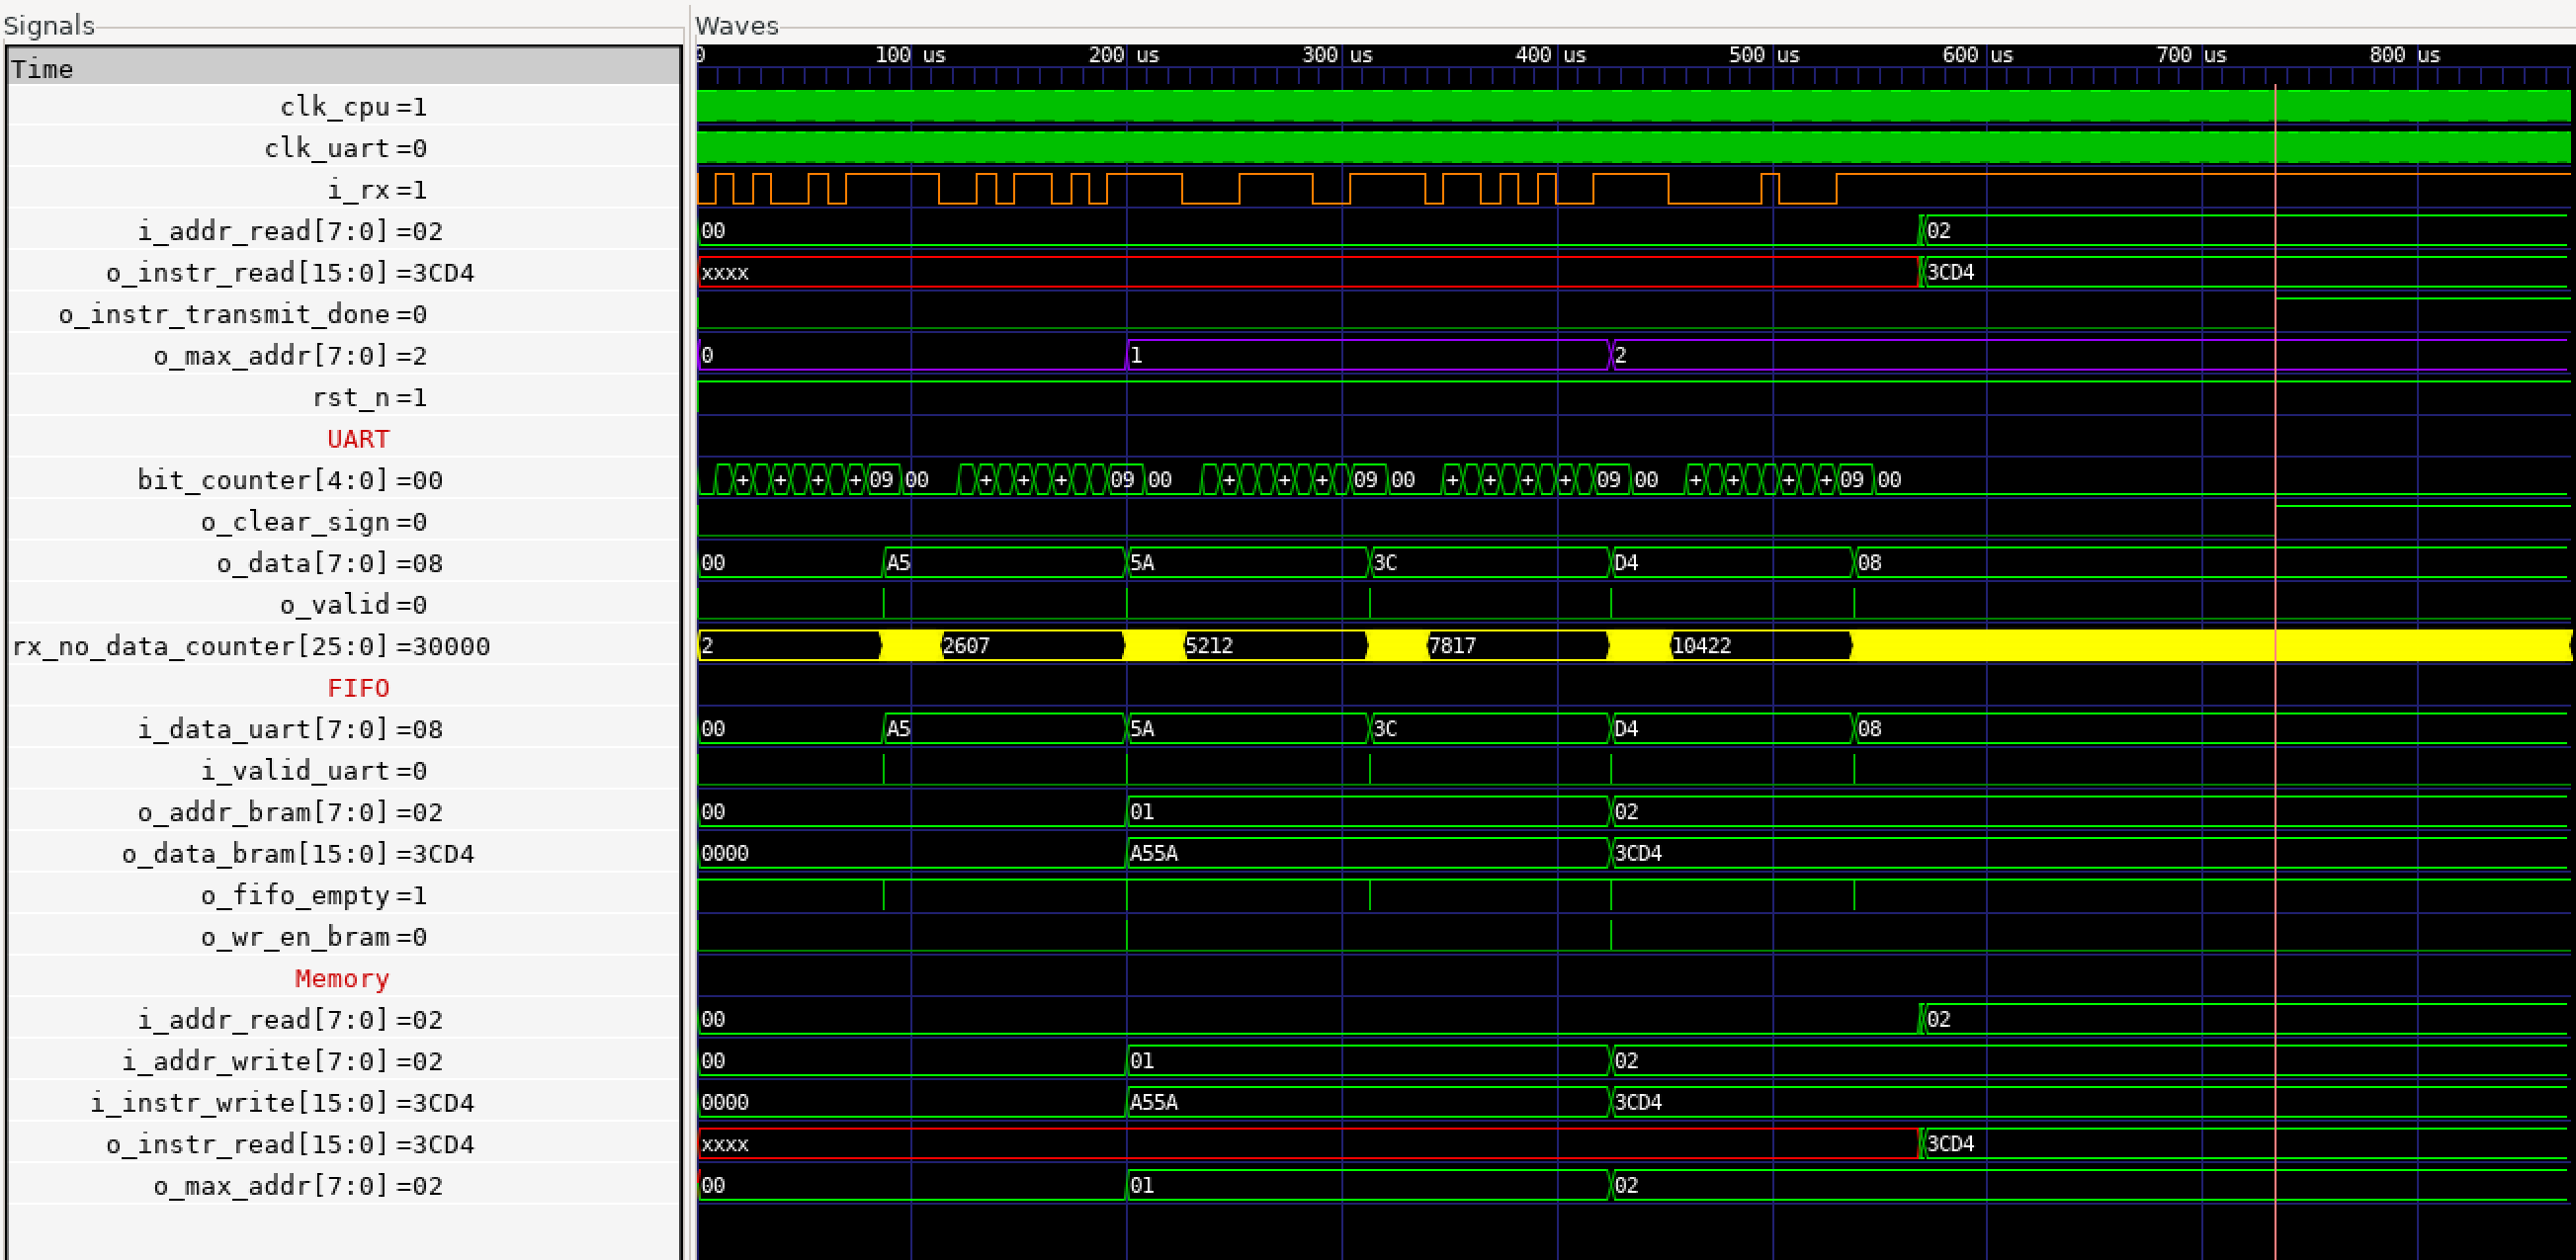
\includegraphics[width = 0.95\textwidth]{figure/instr_rom_sim.png}
  \caption{指令ROM部分仿真}
\end{figure}
\subsection{基础模块设计}
\subsubsection{ALU}
ALU运算结果存放于MR寄存器和ACC寄存器中。其中MR寄存器存放乘法运算的高位结果,ACC寄存器存放乘法运算的低位结果。
\subsubsection{MAR}
\subsubsection{MBR}
\subsubsection{PC}
\subsubsection{IR}
\subsubsection{ACC}
\subsubsection{数据RAM}
\subsubsection{Control Unit}

参考表~\ref{tab:CPU:DataPath}~,确定指令集中的每一条指令对应的控制信号,并存储到CU的内部寄存器中,即可完成CU的主要功能设计。



% \subsection{分支预测}

\section{仿真验证}
\subsection{时延分析}

\subsection{激励设置}

\section{FPGA实现}
\subsection{用户输入端}
采用第一个测试样例进行测试。
$$
1+2+\dots +99 +100 =5050
$$
编写源程序如下:
\begin{lstlisting}[language=Assembly]
      LOAD IMMEDIATE 0 
      STORE 1
      LOAD IMMEDIATE 1
      STORE 2
      LOAD IMMEDIATE 100
      STORE 3
LOOP: LOAD 1
      ADD 2
      STORE 1
      LOAD 2
      ADD IMMEDIATE 1
      STORE 2
      LOAD 2
      SUB 3
      JGZ LOOP

      HALT
\end{lstlisting}
\nocite{FPGA-CPU}
\newpage
\printbibliography
\newpage
\addappheadtotoc
\begin{appendices}
  \section{完整设计代码}
  \subsection{汇编程序处理Python脚本}\label{sec:appendices:python}
  \lstinputlisting[language=python,caption={write\_bistream.py}]{./designs/input_src/write_bitstream.py}
  
\end{appendices}

\end{document}

%! I felt extremely sorry to remove the whole section of Pipeline Design.

% \section{流水线架构与优化策略}
% 参考资料与文献:\cite{hu2024computer}
% \subsection{流水线阶段}
% 为了加速CPU的指令执行速度,采用\textbf{6级同步流水线}完成CPU执行指令的全流程。分别为:取指令(IF),指令译码(ID),取操作数(FO),间址(IND),指令执行(EX)和写回寄存器(WB)六个阶段。流水线的六个阶段如下所示。
% $$
%   \text{IF} \rightarrow \text{ID} \rightarrow \text{FO}\rightarrow \text{IND} \rightarrow \text{EX} \rightarrow \text{WB}
% $$

% 流水线各阶段的主要工作如下:
% \begin{itemize}
%   \item \textbf{IF(Instruction Fetch):}从指令存储器中取出指令,同时确定下一条指令地址(指针指向下一条指令);
%   \item \textbf{ID(Instruction Decode):}翻译指令,同时让计算机得出要使用的寄存器,得出寻址方式,亦或者(转移指令)是给出转移目的寄存器与转移条件;
%   \item \textbf{FO(Fetch Operands):}取立即操作数到MBR,即指令的低8位。
%   \item \textbf{IND(Indirect):}间接寻址周期,每插入一个IND周期则间接寻址深度+1。不插入IND周期则为立即数寻址。在本设计中由于不考虑间接寻址,因此最多只有1个IND周期。\textbf{立即数寻址的指令将跳过这一阶段。}
%   \item \textbf{EX(Execution):}按照微操作指令指示打开数据通路。
%   \item \textbf{WB(Write Back):}将运算结果保存到目标寄存器。
% \end{itemize}

% 因此,对于每一条指令,都会经历上述六个指令周期中的一部分,而由表~\ref{tab:five_stage_pipeline_ctrl}~可知,其中IF和ID部分所有指令公用相同的微操作指令。
% \subsection{流水线寄存器}
% 为了使多条指令各阶段的数据在转换时可以保存,避免出现输出数据被覆盖的情况,需要设立5个流水线寄存器贮存上一阶段的输出。为方便起见,这些寄存器命名统一为“阶段1\_阶段2\_SHIFT\_REG”的方式。

% 每一个寄存器所贮存的内容应当至少支撑起下一阶段的输入,基于此原则,可以给出每个转移寄存器所需贮存的内容如表~\ref{tab:pipeline:shiftreg}。
% \begin{longtable}{c c c}
%   \caption{流水线寄存器功能一览} \label{tab:pipeline:shiftreg} \\
%   \toprule
%   转移寄存器 & 贮存内容(高位到低位)  & 位宽   \\
%   \midrule
%   \endfirsthead

%   \caption[]{(续表)流水线寄存器功能一览} \\
%   \toprule
%   转移寄存器 & 贮存内容  & 位宽  \\
%   \midrule
%   \endhead

%   \midrule
%   \multicolumn{3}{r}{续下页} \\
%   \midrule
%   \endfoot

%   \bottomrule
%   \endlastfoot

%   IF\_ID\_SHIFT\_REG  & PC/MBR   & 8/16  \\
%   ID\_FO\_SHIFT\_REG  & IR    & 16  \\
%   FO\_IND\_SHIFT\_REG  & IR[15:8], MBR[7:0]    & 16  \\
%   IND\_EX\_SHIFT\_REG  & MBR/ACC   & 16/16  \\
%   EX\_WB\_SHIFT\_REG  & BR/MBR/MAR\footnote{根据指令选择存放什么寄存器中的内容,若位宽过剩,默认高位补零。}   & 32  \\
%   % WB\_OUT\_SHIFT\_REG & 指令的输出结果:ACC/MR/Flags & 36

% \end{longtable}

% \subsection{流水线冒险}
% 包含三种冒险情况:结构冒险、数据冒险、控制冒险(分支冒险)。\cite{zhihu453232311}

% 结构冒险,即\textbf{两条指令共同访问了一个外围设备,不支持同时读取/写入的情况。}在本设计中,由于采用哈佛结构,指令ROM和数据RAM分开,并使用不同的数据总线和地址总线,因此不会出现结构冒险。并且,尽管不同运算指令可能会使用相同的寄存器,如MBR,但由于指令不可能同时处于相同的阶段,他们一定会被保存在不同的流水线寄存器中。

% 数据冒险,即\textbf{某指令引用了前一次的运算结果,但其结果值还未产生}。常见的数据冒险包括读后写 (Read After Write),写后读(WAR, Write After Read) 和 写后写(WAW, Write After Write)冲突。在顺序流水线设计中,后两种数据冒险不常见,在本设计中不考虑。

% 控制冒险,即 \textbf{由于程序中存在分支、跳转等控制流改变的指令,导致流水线提前取到的指令可能是错误的}。当遇到分支指令时,流水线可能已经开始执行接下来的几条指令,而此时是否跳转还不确定,如果最终确实发生了跳转,这些指令将被作废,必须清空流水线并从正确的地址重新取指。为了解决控制冒险,本设计中采用了分支预测技术,提前猜测分支是否发生,并按照预测结果继续执行流水线,若预测正确则无需清空流水线,提高了效率;若预测失败,则需要清空错误的指令并重新取指。

% \subsection{数据冒险的解决:前递与旁路}
% 为了解决数据冒险,一般而言采用\textbf{插入空指令(NOP)}的方式。在本设计中,NOP的控制信号为全0,存放于CU的ROM第255个地址处(全1地址)。然而插入空指令降低了流水线的效率,为了提升效率,需要找到更好的解决方式。

% 为了解决RAW数据冒险,
% \subsection{控制冒险的解决:分支预测}
% 在本设计中,为了减少分支指令(JMP,JGZ)带来的流水线Flush和延迟,采用1比特分支预测进行流水线优化。

% 分支预测发生在分支指令执行至\textbf{ID}阶段时。CU在译码后发现其为跳转类指令,就会向Branch Predictor发送一个信号,要求进行分支预测。分支预测的结果决定接下来流水线中IF阶段读取指令的地址,但若在EX阶段发现预测结果和实际结果不一致,则对已抓取的所有指令清空(Flush)。分支预测的具体步骤如算法~\ref{alg:1bitBP}。

% \begin{algorithm}[htbp]
%   \caption{1-bit 分支预测}
%   \label{alg:1bitBP}
%   \begin{algorithmic}[1]
%   \State \textbf{Note:} 使用 1-bit 预测器预测分支是否跳转
%   \State \textbf{Input:} $PC, BranchTaken$
%   \State \textbf{Output:} $NextPC$
%   \State \textbf{Internal Registers:} $PredictorBit, BranchTarget$

%   \Procedure{Branch Prediction}{}
%       \If {$PredictorBit == 1$}
%           \State $PredictedTaken \gets \text{True}$
%           \State $NextPC \gets BranchTarget$
%       \Else
%           \State $PredictedTaken \gets \text{False}$
%           \State $NextPC \gets PC + 1$
%       \EndIf
%   \EndProcedure

%   \Procedure{Branch Resolution}{}
%       \If {$BranchTaken \neq PredictedTaken$}  \Comment{预测错误}
%           \State $Flush \gets 1$  \Comment{清空错误指令}
%           \State $NextPC \gets \textbf{if } BranchTaken \textbf{ then } BranchTarget \textbf{ else } PC + 1$
%       \EndIf
%       \State \textbf{Update Predictor:}
%       \State $PredictorBit \gets BranchTaken$  \Comment{更新 1-bit 预测器}
%   \EndProcedure
%   \end{algorithmic}
% \end{algorithm}

% \begin{figure}[htbp]
%   \centering
%   \caption{流水线优化:前递} \label{fig:pipeline:1}
%   \begin{tikzpicture}[x=0.8cm, y=0.8cm]



%     % % 指令标签
%     \node[anchor=east] at (0.5,-1.5) {\textbf{LOAD}~1};
%     \node[anchor=east] at (0.5,-2.5) {\textbf{ADD}~2};
%     \node[anchor=east] at (0.5,-3.5) {\textbf{ADD}~3};
%     \node[anchor=east] at (0.5,-4.5) {\textbf{STORE}~1};
%     \node[anchor=east] at (0.5,-5.5) {\textbf{SUB}~3};
%     \node[anchor=east] at (0.5,-6.5) {\textit{INSTR\_AFTER}};
    
      
%       % 指令的执行阶段(用方块)
%       \newcommand{\drawstage}[3]{ % #1: x位置,#2: y位置,#3: 字母
%         \draw[fill=blue!20] (#1,-#2) rectangle ++(1,-1);
%         \node at (#1+0.5,-#2-0.5) {\textbf{#3}};
%       }
%       \newcommand{\drawstageorange}[3]{ % #1: x位置,#2: y位置,#3: 字母
%         \draw[fill=orange!20] (#1,-#2) rectangle ++(1,-1);
%         \node at (#1+0.5,-#2-0.5) {\textbf{#3}};
%       }
%       % 手动绘制流水线阶段
%       %              x, y, 阶段
%       \drawstage{1}{1}{I}
%       \drawstage{2}{1}{D}
%       \drawstage{3}{1}{F}
%       \drawstage{4}{1}{N}
%       \drawstage{5}{1}{E}
%       \drawstage{6}{1}{W}
      
%       \drawstage{2}{2}{I}
%       \drawstage{3}{2}{D}
%       \drawstage{4}{2}{F}
%       \drawstage{5}{2}{N}
%       \drawstage{6}{2}{E}
%       \drawstage{7}{2}{W}
      
%       % % Stall 插入
%       % \draw[fill=gray!30] (3,-3) rectangle ++(1,-1);
%       % \node at (3.5,-3.5) {\textbf{Stall}};
%       \drawstage{3}{3}{I}
%       \drawstage{4}{3}{D}
%       \drawstage{5}{3}{F}
%       \drawstage{6}{3}{N}
%       \drawstage{7}{3}{E}
%       \drawstage{8}{3}{W}

%       \drawstage{4}{4}{I}
%       \drawstage{5}{4}{D}
%       \drawstage{6}{4}{F}
%       \drawstage{7}{4}{N}
%       \drawstage{8}{4}{E}
%       \drawstage{9}{4}{W}
      
%       \drawstage{5}{5}{I}
%       \drawstage{6}{5}{D}
%       \drawstage{7}{5}{F}
%       \drawstage{8}{5}{N}
%       \drawstage{9}{5}{E}
%       \drawstage{10}{5}{W}
      
%       % 注释箭头和文字
%       \draw[->, thick, blue] (5.5,-1.5) -- (5.5,-2.2);
%       \draw[->, thick, blue] (6.5,-2.5) -- (6.5,-3.2);
%       \node[anchor=west, font=\small, color = blue] at (8.6,-2) {\makecell{前递:ADD指令的ACC使用\\上一条指令运算结果,EX阶段不再读取}};
      
%       % \draw[->, thick, gray] (3.5,-2.5) -- (3.5,-3.2);
%       % \node[anchor=west, font=\small, color = gray] at (8.6,-1.75) {Stall:等待LOAD结果};
      

      
%       \end{tikzpicture}
% \end{figure}

% \begin{figure}[htbp]
%   \centering
%   \caption{流水线优化:分支预测} \label{fig:pipeline:example}
%   \begin{tikzpicture}[x=0.8cm, y=0.8cm]



%     % % 指令标签
%     \node[anchor=east] at (0.5,-1.5) {\textbf{LOAD}~1};
%     \node[anchor=east] at (0.5,-2.5) {\textbf{ADD}~2};
%     % \node[anchor=east] at (0.5,-3.5) {\textit{STALL}};
%     \node[anchor=east] at (0.5,-3.5) {\textbf{STORE}~1};
%     \node[anchor=east] at (0.5,-4.5) {\textbf{SUB}~3};
%     \node[anchor=east] at (0.5,-5.5) {\textbf{JGZ}~LOOP};
%     \node[anchor=east] at (0.5,-6.5) {\textit{INSTR\_AFTER}};
%     \node[anchor=east] at (0.5,-7.5) {\textit{(FLUSH)}};
    
      
%       % 指令的执行阶段(用方块)
%       \newcommand{\drawstage}[3]{ % #1: x位置,#2: y位置,#3: 字母
%         \draw[fill=blue!20] (#1,-#2) rectangle ++(1,-1);
%         \node at (#1+0.5,-#2-0.5) {\textbf{#3}};
%       }
%       \newcommand{\drawstageorange}[3]{ % #1: x位置,#2: y位置,#3: 字母
%         \draw[fill=orange!20] (#1,-#2) rectangle ++(1,-1);
%         \node at (#1+0.5,-#2-0.5) {\textbf{#3}};
%       }
%       % 手动绘制流水线阶段
%       %              x, y, 阶段
%       \drawstage{1}{1}{I}
%       \drawstage{2}{1}{D}
%       \drawstage{3}{1}{F}
%       \drawstage{4}{1}{N}
%       \drawstage{5}{1}{E}
%       \drawstage{6}{1}{W}
      
%       \drawstage{2}{2}{I}
%       \drawstage{3}{2}{D}
%       \drawstage{4}{2}{F}
%       \drawstage{5}{2}{N}
%       \drawstage{6}{2}{E}
%       \drawstage{7}{2}{W}
      
%       % Stall 插入
%       % \draw[fill=gray!30] (3,-3) rectangle ++(1,-1);
%       % \node at (3.5,-3.5) {\textbf{Stall}};
%       \drawstage{3}{3}{I}
%       \drawstage{4}{3}{D}
%       \drawstage{5}{3}{F}
%       \drawstage{6}{3}{N}
%       \drawstage{7}{3}{E}
%       \drawstage{8}{3}{W}

%       \drawstage{4}{4}{I}
%       \drawstage{5}{4}{D}
%       \drawstage{6}{4}{F}
%       \drawstage{7}{4}{N}
%       \drawstage{8}{4}{E}
%       \drawstage{9}{4}{W}
      
%       \drawstage{5}{5}{I}
%       \drawstageorange{6}{5}{D}
%       \drawstage{7}{5}{F}
%       \drawstage{8}{5}{N}
%       \drawstage{9}{5}{E}
%       \drawstage{10}{5}{W}

%       \drawstage{6}{6}{I}
%       \drawstage{7}{6}{D}
%       \drawstage{8}{6}{F}
%       \drawstage{7}{7}{I}
%       \drawstage{8}{7}{D}
%       \drawstage{8}{8}{I}
%       % \drawstage{6}{6}{I}
%       % \drawstageorange{7}{6}{D}
%       % \drawstage{8}{6}{F}
%       % \drawstage{9}{6}{N}
%       % \drawstage{10}{6}{E}
%       % \drawstage{11}{6}{W}
      
%       % Flush显示
%       \foreach \i in {9,10,11} {
%         \draw[fill=red!20] (\i,-6) rectangle ++(1,-1);
%         \node at (\i+0.5,-6.5) {X};
%       }
%       \foreach \i in {9,10,11,12} {
%         \draw[fill=red!20] (\i,-7) rectangle ++(1,-1);
%         \node at (\i+0.5,-7.5) {X};
%       }
%       \foreach \i in {9,10,11,12,13} {
%         \draw[fill=red!20] (\i,-8) rectangle ++(1,-1);
%         \node at (\i+0.5,-8.5) {X};
%       }
%       % 注释箭头和文字
      
%       % \draw[->, thick, orange] (9.5,-5.5) -- (9.5,-6.2);
%       % \node[anchor=west, font=\small,color = orange] at (8.6,-2.5) { 分支预测:假设跳转};
      
%       \draw[->, thick, red] (9.5,-5.5) -- (9.5,-6.2);
%       % \node[anchor=west, font=\small,color = red] at (8.6,-3.25) { Flush:跳转错误清空};
      
%       \end{tikzpicture}
% \end{figure}
% tikz 流水线图
% \begin{figure}[htbp]
%   \centering
%   \caption{流水线优化策略举例} \label{fig:pipeline:example}
%   \begin{tikzpicture}[x=0.8cm, y=0.8cm]



%     % % 指令标签
%     \node[anchor=east] at (0.5,-1.5) {\textbf{LOAD}~1};
%     \node[anchor=east] at (0.5,-2.5) {\textbf{ADD}~2};
%     \node[anchor=east] at (0.5,-3.5) {\textit{STALL}};
%     \node[anchor=east] at (0.5,-4.5) {\textbf{STORE}~1};
%     \node[anchor=east] at (0.5,-5.5) {\textbf{SUB}~3};
%     \node[anchor=east] at (0.5,-6.5) {\textbf{JGZ}~LOOP};
%     \node[anchor=east] at (0.5,-7.5) {\textit{INSTR\_AFTER}};
%     \node[anchor=east] at (0.5,-8.5) {\textit{(FLUSH)}};
    
      
%       % 指令的执行阶段(用方块)
%       \newcommand{\drawstage}[3]{ % #1: x位置,#2: y位置,#3: 字母
%         \draw[fill=blue!20] (#1,-#2) rectangle ++(1,-1);
%         \node at (#1+0.5,-#2-0.5) {\textbf{#3}};
%       }
%       \newcommand{\drawstageorange}[3]{ % #1: x位置,#2: y位置,#3: 字母
%         \draw[fill=orange!20] (#1,-#2) rectangle ++(1,-1);
%         \node at (#1+0.5,-#2-0.5) {\textbf{#3}};
%       }
%       % 手动绘制流水线阶段
%       %              x, y, 阶段
%       \drawstage{1}{1}{I}
%       \drawstage{2}{1}{D}
%       \drawstage{3}{1}{F}
%       \drawstage{4}{1}{N}
%       \drawstage{5}{1}{E}
%       \drawstage{6}{1}{W}
      
%       \drawstage{2}{2}{I}
%       \drawstage{3}{2}{D}
%       \drawstage{4}{2}{F}
%       \drawstage{5}{2}{N}
%       \drawstage{6}{2}{E}
%       \drawstage{7}{2}{W}
      
%       % Stall 插入
%       \draw[fill=gray!30] (3,-3) rectangle ++(1,-1);
%       \node at (3.5,-3.5) {\textbf{Stall}};
      
%       \drawstage{4}{4}{I}
%       \drawstage{5}{4}{D}
%       \drawstage{6}{4}{F}
%       \drawstage{7}{4}{N}
%       \drawstage{8}{4}{E}
%       \drawstage{9}{4}{W}
      
%       \drawstage{5}{5}{I}
%       \drawstage{6}{5}{D}
%       \drawstage{7}{5}{F}
%       \drawstage{8}{5}{N}
%       \drawstage{9}{5}{E}
%       \drawstage{10}{5}{W}
      
%       \drawstage{6}{6}{I}
%       \drawstageorange{7}{6}{D}
%       \drawstage{8}{6}{F}
%       \drawstage{9}{6}{N}
%       \drawstage{10}{6}{E}
%       \drawstage{11}{6}{W}
      
%       % Flush显示
%       \foreach \i in {7,8,9,10,11,12} {
%         \draw[fill=red!20] (\i,-7) rectangle ++(1,-1);
%         \node at (\i+0.5,-7.5) {X};
%       }
      
%       % 注释箭头和文字
%       \draw[->, thick, blue] (5.5,-1.5) -- (5.5,-2.2);
%       \node[anchor=west, font=\small, color = blue] at (8.6,-1) {前递:ADD使用LOAD结果};
      
%       \draw[->, thick, gray] (3.5,-2.5) -- (3.5,-3.2);
%       \node[anchor=west, font=\small, color = gray] at (8.6,-1.75) {Stall:等待LOAD结果};
      
%       % \draw[->, thick, orange] (9.5,-5.5) -- (9.5,-6.2);
%       \node[anchor=west, font=\small,color = orange] at (8.6,-2.5) { 分支预测:假设跳转};
      
%       \draw[->, thick, red] (10.5,-6.5) -- (10.5,-7.2);
%       \node[anchor=west, font=\small,color = red] at (8.6,-3.25) { Flush:跳转错误清空};
      
%       \end{tikzpicture}
% \end{figure}